\section{Interface Signals}
\label{sec:is}

The interface signals of the Versat controller core are described in Table~\ref{tab:is}.

\begin{table}[h]
\centering
\begin{tabular}{|l|c|l|}
\hline
\multicolumn{1}{|c|}{\bf Name} & {\bf Direction} & \multicolumn{1}{c|}{\bf Description} \\ 
\hline \hline
\multicolumn{1}{|l|}{clk}                & IN    & Clock signal.\\ 
\hline
\multicolumn{1}{|l|}{rst}                & IN    & \multicolumn{1}{l|}{Reset signal.}\\
\hline \hline
\multicolumn{3}{|c|}{{\bf Instruction Bus Interface}}\\ 
\hline \hline
instruction[31:0]                        & IN    & Instruction to execute.\\ 
\hline
pc[9:0]                                  & OUT   & Program Counter (instruction address).\\ 
\hline \hline
\multicolumn{3}{|c|}{{\bf Data Bus Interface}}\\ 
\hline \hline
data\_sel                                & OUT   & Read or write request.\\ 
\hline
data\_we                                 & OUT   & Write enable.\\ 
\hline
data\_addr[9:0]                          & OUT   & Data address.\\ 
\hline
data\_to\_rd[31:0]                       & IN    & Data to be read.\\ 
\hline
data\_to\_wr[31:0]                       & OUT   & Data to be written. \\ 
\hline
\end{tabular}
\caption{Interface signals.}
\label{tab:is}
\end{table}

\subsection{Instruction Bus Timing Diagram}
\label{sec:instrird}

The timing diagram for an instruction read transaction is shown in
Figure~\ref{fig:instrird}.

\begin{figure}[htbp]
    \centerline{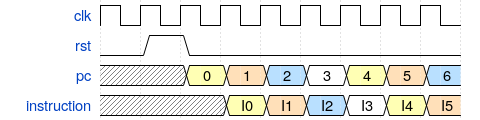
\includegraphics[width=.8\textwidth]{instr_rd}}
    \vspace{0cm}\caption{Instruction (pipelined) reads.}
    \label{fig:instrird}
\end{figure}

\subsection{Data Bus Timing Diagram}
\label{sec:rwi}

The timing diagrams for data reads and writes are shown in
Figure~\ref{fig:rwird} and Figure~\ref{fig:rwiwr}, respectively. These
operations may be consecutive or not, as illustrated.

\begin{figure}[htbp]
    \centerline{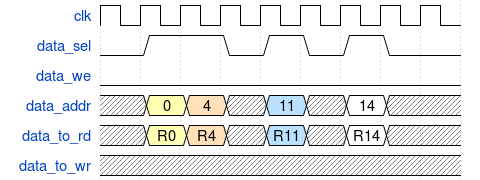
\includegraphics[width=.8\textwidth]{rw_rd}}
    \vspace{0cm}\caption{Data Bus reads.}
    \label{fig:rwird}
\end{figure}

\begin{figure}[htbp]
    \centerline{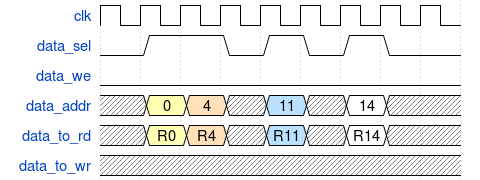
\includegraphics[width=.8\textwidth]{rw_wr}}
    \vspace{0cm}\caption{Data Bus writes.}
    \label{fig:rwiwr}
\end{figure}

